\documentclass[11pt]{article}

\usepackage{authblk}
\usepackage{setspace} 
\usepackage{lineno} 
\usepackage[a4paper, margin=2cm]{geometry} 
\usepackage[parfill]{parskip}
\usepackage{graphicx} 
\usepackage[section]{placeins} 

% Harvard-style referencing
\usepackage[comma]{natbib}
\bibliographystyle{agsm}
\setcitestyle{authoryear,open={(},close={)}}

% line numbering
\doublespacing

\title{\textbf{Plant Stress Detection Based on Spectral Imaging and Deep Learning}}
\author[]{Xiaosheng Luo}
\affil[]{Imperial College London}
\date{}


\begin{document}
  \maketitle

\section*{}
\begin{center}
	\textbf{Supervisor:} Oliver Windram, Department of Life Sciences (Silwood Park), Imperial College London
\end{center}


\newpage
\section*{Introduction}
\begin{linenumbers}
Organic growers face a number of challenges they must overcome to deliver high quality food to their customers. The lack of reactive chemical control measures in organic farming requires additional levels of insight in order to optimise plant and hervest schedule. Traditional manual detection can only wait until late crop stress morphological changes, and is generally time-consuming and subjective. However, using spectral imaging technology, the differences in crop physiological structure characteristics will lead to differences in light reflection, absorption and transmission. Studying these differences in spectral imaging can help identify the crop growth status, nutrient and disease.

Previous studies have made extensive fundamental research on crop detection using spectral technology, mainly based on spectral index features and image features. For instance, the olive Verticillium wilt can be diagnosed by images collected from UAV-mounted multi-spectral camera and thermal infrared camera, and it was found that early Verticillium wilt was related to green light band, and chlorophyll fluorescence index decreased with the disease aggravating \citep{calderon2013high}. Moreover, applied hyperspectral imaging techniques to identify the angular leaf spot of cucumber by detecting the contents of chlorophyll and carotenoids showed the feasible for visualizing the pigment distribution in cucumber leaves in response to angular leaf spot \citep{zhao2016hyperspectral}. Besides, progress has also been made in the research of crop identification \citep{torres2013imagery,laliberte2009texture}, as well as crop growth status monitoring \citep{vega2015multi}.

Although the identification of different plant stresses has reached a considerable level of accuracy, the pratical plant stress process may be more complicated and the understanding of the spectral images of plant stress could be deeper. In order to explore the feasibility of using spectral imaging to identify complex plant stress and better apply spectroscopy technology to pratical production, we propose the application and research and as follow: 
\begin{itemize} 
	\item [1)] How can we build a robust classifier to detecte the quality of organically grown broccoli on conveyor belts using spetral imaging? 
	\item [2)] Can we build a robust classifier based on limited data set, using the spectral images collected under different combinations of stress (temperature, light, drought)? How can we extend to the field?
	\item [3)] Deep into a metabolic levels, can we find the evidence to support the classification?
\end{itemize}
\end{linenumbers}

\title{\textbf{keywords:} Organic farming, Deep learning, Plant stress, Spectral imaging, Detection, Metabolomics

\section*{Methods}
\begin{linenumbers}
First, use multi-spectral imaging technology combined with deep learning algorithms to detecte the quality of organically grown broccoli on conveyor belts. 

Second, build the same detection model using the data collected by the drone.

Third, under the environment controlled by the laboratory, collect spectral image data under different combinations of stress (temperature, light, drought) and explore the possibility of establishing a robust classifier in a limited data set. 

Fourth, sample and explore molecular differences by GC-MS, to provide classification basis in metabolic levels. 
\end{linenumbers}

\section*{Expected Outcomes}
\begin{linenumbers}
Robust spectral images classifiers and matabolomics analysis.
\end{linenumbers}

\section*{Budget}
\begin{linenumbers}
\pounds 500 funded by school for computing hours, printing costs and for travel related to the project.
\end{linenumbers}

\section*{Project Feasibility}
\begin{linenumbers}
Feasible equipment for data collecting and timeline as bellow
\end{linenumbers}


\begin{figure}[!ht]
	\centering
	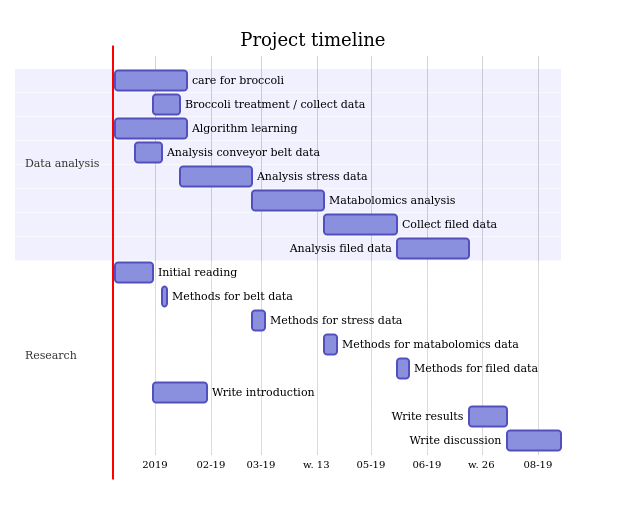
\includegraphics[scale=0.5]{./gantt.png} 
\end{figure}


\bibliography{Proposal}
\end{document}